\documentclass{math}

\usepackage{circuitikz}
\usepackage{tikz}

\title{University Physics 2}
\author{Alvin Lin}
\date{January 2018 - May 2018}

\begin{document}

\maketitle

\section*{Circuits}
We will start with a microscopic pictures of current and resistance.
\begin{center}
  \begin{circuitikz}
    \draw (0,0) to[battery, l=\( \Delta V \)] (0,2) -- (4,2)
      to[resistor, l=R] (4,0) -- (0,0);
   \draw[->] (1.5,2.5) -- (2.5,2.5) node[pos=0.5,above] {\( I \)};
  \end{circuitikz}
\end{center}
Current will flow clockwise in this example, from the positive terminal of the
battery through the wires, into the negative terminal. If we look at a small
section of wire at the top.
\begin{center}
  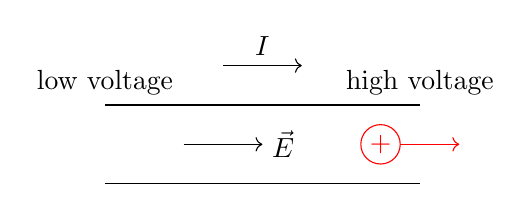
\begin{tikzpicture}
    \draw (0,0) -- (4,0);
    \draw (0,1) node[above] {low voltage} -- (4,1) node[above] {high voltage};
    \draw[->] (1.5,1.5) -- (2.5,1.5) node[pos=0.5,above] {\( I \)};
    \draw[->] (1,0.5) -- (2,0.5) node[right] {\( \vec{E} \)};
    \draw[red] (3.5,0.5) circle (0.25) node[] {+};
    \draw[red,->] (3.75,0.5) -- (4.5,0.5);
  \end{tikzpicture}
\end{center}
We define current, \( I \) as the charge moved through the wire, per unit time.
\[ I = \ddiff{Q}{t} = nqAV_d \]
Sometimes, we will want the current density:
\[ J = \frac{I}{A} = nqV_d \]
All the constants can be defined and rewritten:
\[ \rho = \frac{E}{J} \]
where \( \rho \) is the resistivity of the wire. It is a fundamental property of
a material independent of area or density.
\[ [\rho] = \frac{[E]}{[J]} = \frac{\frac{V}{m}}{\frac{A}{m^2}} =
  \frac{V\cdot m}{A} \]
\begin{align*}
  E &= \rho J \\
  EL &= \rho JL \\
  \Delta V &= \frac{\rho IL}{A} \\
  &= \frac{\rho L}{A}I \\
  R &= \frac{\rho L}{A} \\
  \Delta V &= IR
\end{align*}
This is known as Ohm's Law, where the units of resistance \( R \) are measured
in ohms (\( \Omega \)). All these derivations are done in terms of a positive
charge, but in a wire, the charges that are moving are electrons.
\begin{center}
  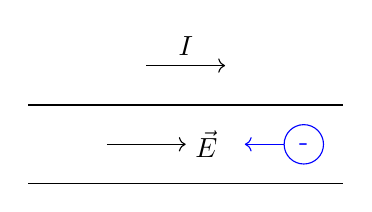
\begin{tikzpicture}
    \draw (0,0) -- (4,0);
    \draw (0,1) -- (4,1);
    \draw[->] (1.5,1.5) -- (2.5,1.5) node[pos=0.5,above] {\( I \)};
    \draw[->] (1,0.5) -- (2,0.5) node[right] {\( \vec{E} \)};
    \draw[blue] (3.5,0.5) circle (0.25) node[] {-};
    \draw[blue,->] (3.25,0.5) -- (2.75,0.5);
  \end{tikzpicture}
\end{center}

\subsection*{Temperature Dependence of Resistance}
Resistivity depends on temperature:
\[ (\rho-\rho_{\circ}) = \rho_{\circ}\alpha(T-T_{\circ}) \]
where \( \rho \) is resistivity, \( T \) is temperature, \( \alpha \) is the
temperature coefficient, and \( T_{\circ},\rho_{\circ} \) are reference values.
Note that this is similar to the equation of a line. Thus, the temperature
coefficient can be determined by measuring these values and determining the
slope of the line plotted by the resistivity at certain temperatures.

\subsection*{Power}
Power is energy per unit time. Recall that current is change in current over
unit time.
\[ I = \frac{\Delta Q}{\Delta t} \quad \Delta Q = I\Delta t \]
With potential energy:
\begin{align*}
  \Delta U &= \Delta QV \\
  \Delta U &= I\Delta tV \\
  \frac{\Delta U}{\Delta t} &= IV \\
  P &= IV
\end{align*}
In relation to Ohm's Law:
\[ P = IV = I^2R = \frac{V^2}{R} \]

\subsection*{Equivalent Resistance (In Series)}
\begin{center}
  \begin{circuitikz}
    \draw (0,0) to[battery, l=\( \Delta V \)] (0,2)
      to[resistor,label=\( R_1 \)] (2,2)
      to[resistor,label=\( R_2 \)] (4,2) -- (4,0) -- (0,0);
  \end{circuitikz} \\[1cm]
  \begin{circuitikz}
    \draw (0,0) to[battery, l=\( \Delta V \)] (0,2)
      to[resistor,label=\( R_{eq} \)] (4,2) -- (4,0) -- (0,0);
  \end{circuitikz}
\end{center}
From conservation of charge:
\[ I_1 = I_2 = I_{eq} \]
From conservation of energy and the equivalent circuit:
\[ \Delta V = \Delta V_1+\Delta V_2 \]
From the equivalent circuit:
\begin{align*}
  \Delta V &= IR_{eq} \\
  \Delta V_1+\Delta V_2 &= IR_{eq}
\end{align*}
Using Ohm's Law:
\begin{align*}
  IR_1+IR_2 &= IR_{eq} \\
  R_1+R_2 &= R_{eq}
\end{align*}
Compared to capacitance:
\[ \frac{1}{C_{eq}} = \frac{1}{C_1}+\frac{1}{C_2} \]

\subsection*{Equivalent Resistance (In Parallel)}
\begin{center}
  \begin{circuitikz}
    \draw (0,0) to[battery, l=\( \Delta V \)] (0,2) -- (2,2)
      to[resistor,label=\( R_1 \)] (2,0) -- (0,0);
    \draw (2,2) -- (4,2)
      to[resistor,label=\( R_2 \)] (4,0) -- (2,0);
  \end{circuitikz} \\[1cm]
  \begin{circuitikz}
    \draw (0,0) to[battery, l=\( \Delta V \)] (0,2) -- (2,2)
      to[resistor,label=\( R_{eq} \)] (2,0) -- (0,0);
  \end{circuitikz}
\end{center}
From conservation of energy:
\[ \Delta V = \Delta V_1 = \Delta V_2 \]
From conservation of charge:
\[ I = I_1+I_2 \]
Using Ohm's Law:
\begin{align*}
  \frac{\Delta V}{R_{eq}} &= \frac{\Delta V}{R_1}+\frac{\Delta V}{R_2} \\
  \frac{1}{R_{eq}} &= \frac{1}{R_1}+\frac{1}{R_2} \\
  R_{eq} &= \frac{R_1R_2}{R_1+R_2}
\end{align*}


\begin{center}
  You can find all my notes at \url{http://omgimanerd.tech/notes}. If you have
  any questions, comments, or concerns, please contact me at
  alvin@omgimanerd.tech
\end{center}

\end{document}
